\FloatBarrier
\section{Inference Evaluation}
\label{sec:inf_eval}

Making situational inferences from partial information is an important downstream use case of schemas. In addition to evaluating the quality of the steps of learned schemas in an ungrounded setting, we evaluate the quality of inferences made about unseen stories using learned schemas. As shown in Figures~\ref{fig:step_inf_eval}~and~\ref{fig:role_inf_eval}, we generate and evaluate two kinds of inferences: \textbf{step inferences}, in which steps from a learned schema are inferred on the basis of having their arguments bound by another, matched step; and \textbf{role inferences}, in which the types of entities are inferred when those entities are bound to arguments in a matched step. Inferred steps are presented to evaluators as tabreps, and inferred roles are presented by filling in the slots in the template sentence ``\textit{In this} \texttt{SCHEMA\_TOPIC} \textit{scenario, the entity} \texttt{ENTITY} \textit{has the role} \texttt{TYPE}.'' For step inferences, two evaluators were presented with three 1-5 Likert scales: one evaluating the \textit{clarity} of the tabrep; one evaluating the \textit{plausibility} of the inference; and one evaluating the \textit{relevance} of the inference, i.e., the degree to which making the inference demonstrates substantial knowledge of the underlying situation. For role inferences, the evaluators received the same Likert scales, with the exception of the \textit{clarity} scale, due to the constrained nature of the template sentence being evaluated.

\subsection{Datasets}
Two datasets are involved in the inference experiment: the set of schemas learned by NESL, and the set of unseen stories for which inferences will be drawn from the corresponding learned schemas. As this experiment only tests inference, and not schema identification, each learned schema is only used to draw inferences on a story that is known to fit the schema's topic already. In order to ensure the unseen stories conceptually fit the schemas, we draw them from the same LSS distribution---modeled by GPT-J 6B---as the stories used for the initial schema learning. In other words, we sample $N+1$ stories during LSS, learn schemas from the first $N$ using NESL, and draw inferences on the final, held-out story for evaluation.

Like in the ungrounded schema evaluation experiment, a research assistant filtered sensible story topics produced by a prompt-based ROCstory summarization model; the 42 schema topics thus chosen are as follows:

\scalebox{0.75}{
\vbox{
\begin{multicols}{3}
\begin{itemize}
\footnotesize
\item \texttt{being in a boat}
\item \texttt{breaking an arm}
\item \texttt{casino}
\item \texttt{church}
\item \texttt{coming home late}
\item \texttt{dogsitting}
\item \texttt{doing homework}
\item \texttt{driving}
\item \texttt{eating at a restaurant}
\item \texttt{eating with friends}
\item \texttt{falling down}
\item \texttt{farming}
\item \texttt{feeling sick}
\item \texttt{flying in an airplane}
\item \texttt{freezing weather}
\item \texttt{getting a haircut}
\item \texttt{giving medicine}
\item \texttt{giving someone a ride}
\item \texttt{going to work}
\item \texttt{growing older}
\item \texttt{having a party}
\item \texttt{having children}
\item \texttt{having pets}
\item \texttt{ice skating}
\item \texttt{jail time}
\item \texttt{jogging}
\item \texttt{meeting new people}
\item \texttt{moving into a new house}
\item \texttt{planting a tree}
\item \texttt{playing an instrument}
\item \texttt{playing in the sand}
\item \texttt{reading a book}
\item \texttt{seeing someone you know}
\item \texttt{sleeping}
\item \texttt{starting a family}
\item \texttt{swimming}
\item \texttt{training an animal}
\item \texttt{traveling}
\item \texttt{waking up}
\item \texttt{walking a dog}
\item \texttt{watching a show}
\item \texttt{working out}
\end{itemize}
\end{multicols}
}
}

\begin{figure}
    \centering
    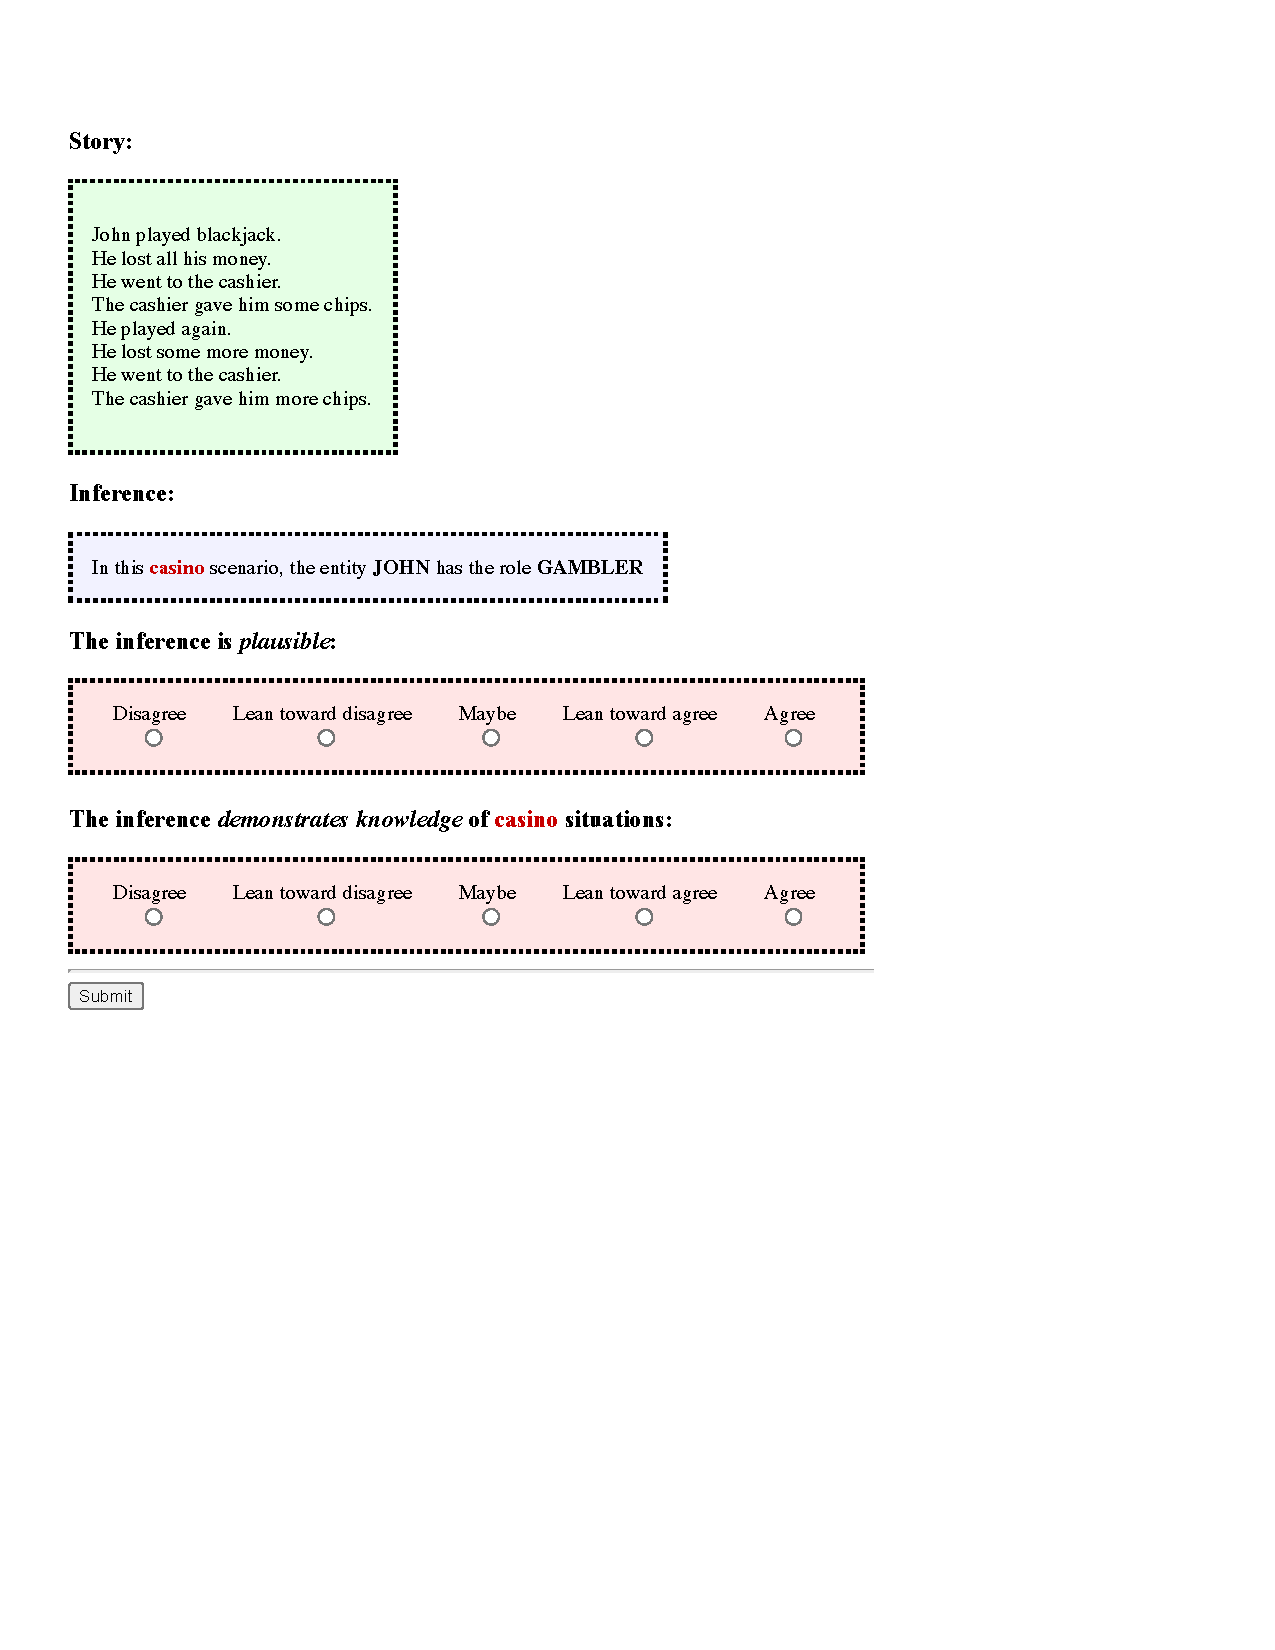
\includegraphics[width=0.5\textwidth]{CH5_eval/role_inf.pdf}
    \caption{An example of a form presented to a schema quality evaluator for a \textit{goal} formula.}
    \label{fig:role_inf_eval}
        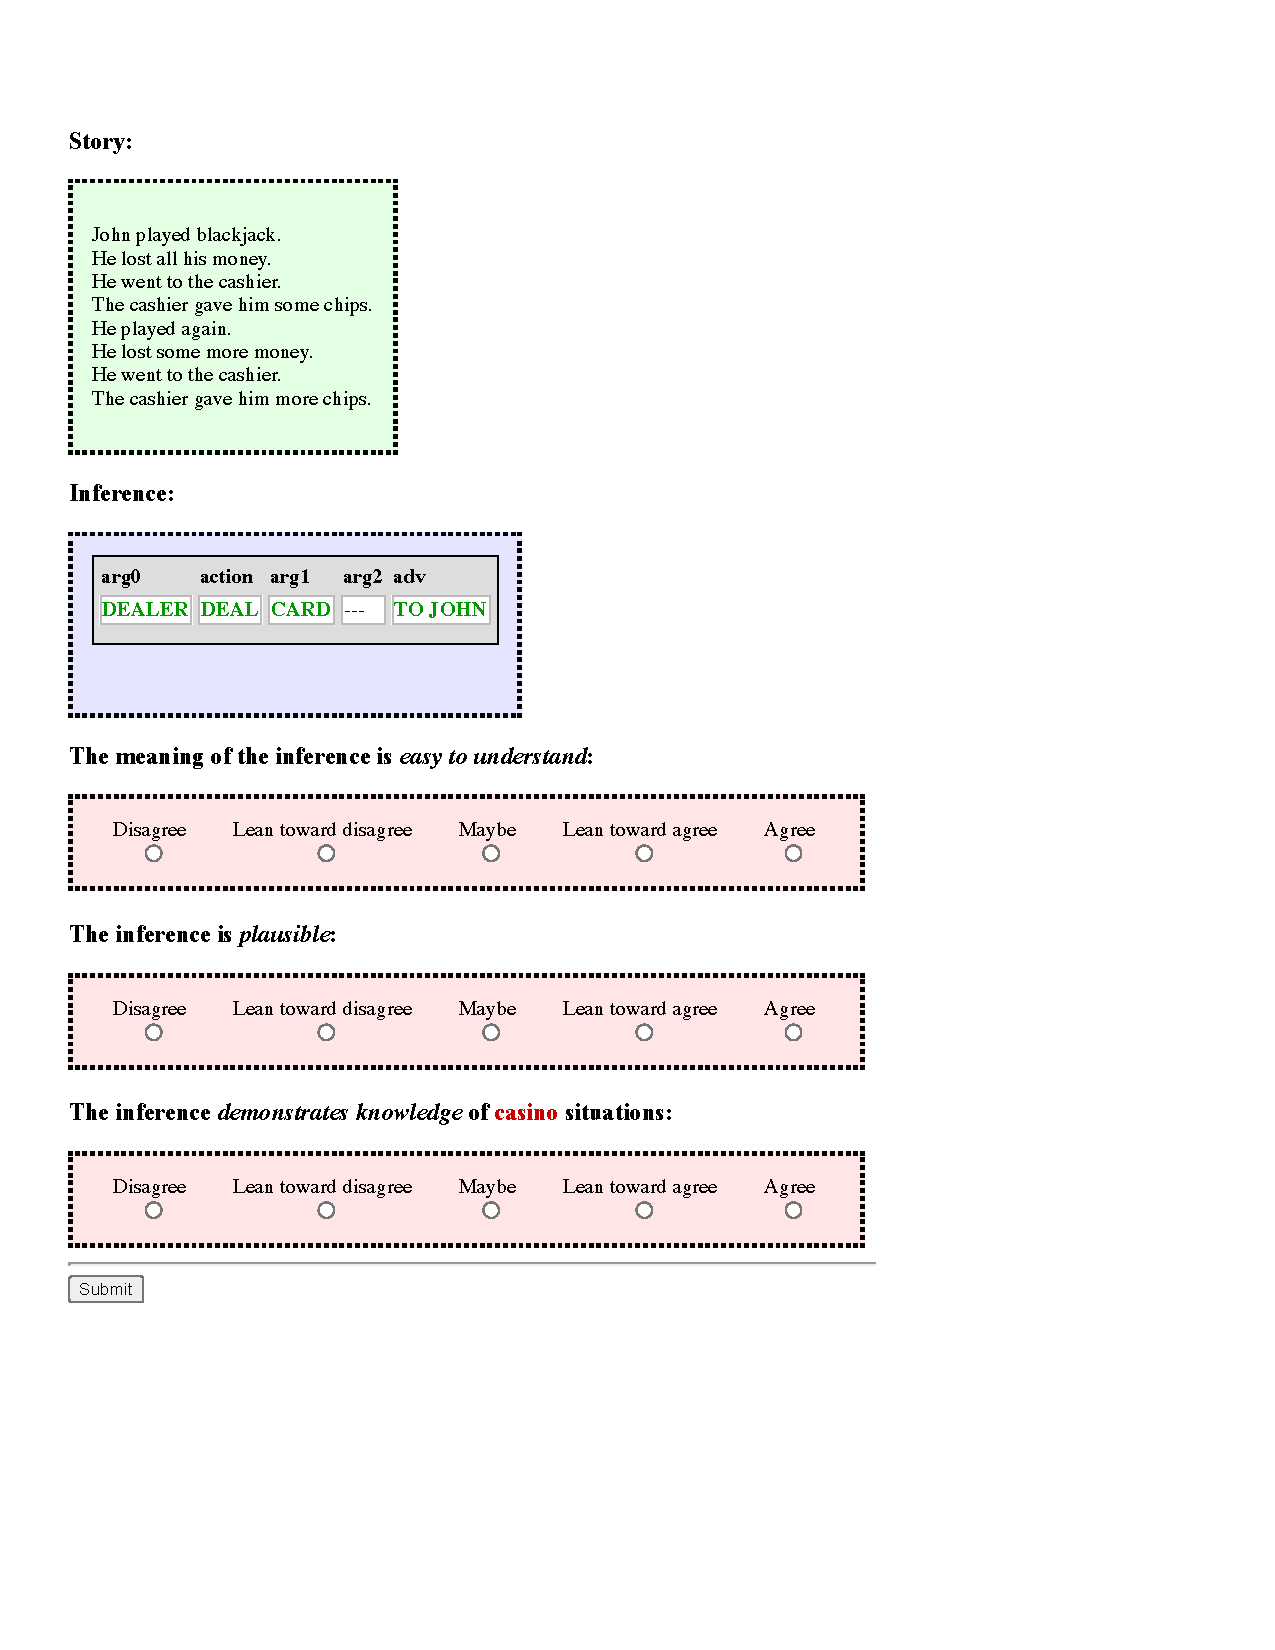
\includegraphics[width=0.5\textwidth]{CH5_eval/step_inf.pdf}
    \caption{An example of a form presented to a schema quality evaluator for a \textit{goal} formula.}
    \label{fig:step_inf_eval}
\end{figure}

\subsection{Results}
\begin{table}[ht]
    \centering
    \begin{tabular}{l|l|l}
       \textbf{Metric} & \textbf{Average Step Score} & \textbf{Average Role Score} \\
       \hline
       Clarity & 0.79 & --- \\
       Plausibility & 0.61 & 0.78 \\
       Relevance & 0.57 & 0.66
    \end{tabular}
    \caption{Average quality scores for inferences about unseen stories generated by learned schemas and presented as tabreps (for steps). Scores have been normalized to a 0-1 range. No clarity measurements were performed for role inferences due to their constrained display representation.}
    \label{tab:inf_results}
\end{table}

We present the results of the grounded schema inference evaluation study in Table~\ref{tab:inf_results}. The clarity of predicted steps is rated fairly highly. Only tabrep visualizations of the formulas were evaluated, but we hypothesize that the pattern of higher ratings of the respective GPT-2 re-verbalizations would hold similarly here, as the formulas being verbalized are the same other than their filled-in values. The plausibility of predicted role types is notably higher than that of predicted steps, perhaps due to the simpler nature of the problem of type assignment relative to that of event prediction. The topical relevance scores of each kind of prediction are significantly lower than the respective plausibility scores, with the relevance-plausibility gap being larger in the case of role type predictions. We interpret this to mean that more plausibly predicted role types are uninteresting or obvious, e.g. \el{PERSON.N}, than plausibly predicted steps. 
The low relevance and probability scores for steps stand in contrast to the relatively higher scores in the ungrounded schema inference evaluation described in Section~\ref{sec:schema_eval}. One possible explanation for the lower plausibility is that predictions are more likely to be wrong when in the context of an entire story, rather than just a topic description, due to increased number of contextual constraints. While relevance was not explicitly worded into the KNEXT-style question of the ungrounded experiment, we find that the relevance and plausibility scores are highly correlated in the grounded inference experiment, with a Pearson correlation coefficient of $\rho = 0.873$. One possible explanation of the low relevance scores, then, is that implausible formulas may, using the wording of the question posted to evaluators, ``demonstrate [less] knowledge'' than plausible ones.

Despite their generally lower values than those in the ungrounded experiment, the plausibility and relevance scores here indicate an average tendency for annotators to agree that the inferences generated by NESL schemas are both plausible and relevant, especially in the case of entity type prediction. That these inferences are the result of an interpretable, deterministic knowledge representation that can be edited is also notable: \citet{weber2022human} have already explored human alterations of learned scripts, reinforcing the importance of human-in-the-loop knowledge \textit{refinement} as a desirable feature of a knowledge representation.